\documentclass{article}

\usepackage[submission]{aaai25}  % DO NOT CHANGE THIS
\usepackage{times}  % DO NOT CHANGE THIS
\usepackage{helvet}  % DO NOT CHANGE THIS
\usepackage{courier}  % DO NOT CHANGE THIS
\usepackage[hyphens]{url}  % DO NOT CHANGE THIS
\usepackage{graphicx} % DO NOT CHANGE THIS
\urlstyle{rm} % DO NOT CHANGE THIS
\def\UrlFont{\rm}  % DO NOT CHANGE THIS
\usepackage{natbib}  % DO NOT CHANGE THIS AND DO NOT ADD ANY OPTIONS TO IT
\usepackage{caption} % DO NOT CHANGE THIS AND DO NOT ADD ANY OPTIONS TO IT
\frenchspacing  % DO NOT CHANGE THIS
\setlength{\pdfpagewidth}{8.5in} % DO NOT CHANGE THIS
\setlength{\pdfpageheight}{11in} % DO NOT CHANGE THIS
%
% These are recommended to typeset algorithms but not required. See the subsubsection on algorithms. Remove them if you don't have algorithms in your paper.
\usepackage{algorithm}
\usepackage{algorithmic}
\usepackage{amsmath}
\usepackage{amsfonts}
\usepackage{amsthm}
\usepackage{mathrsfs}
\usepackage{mathtools}
\usepackage{booktabs}
\usepackage{lipsum}
\usepackage{listings}
\usepackage[acronym]{glossaries}
\usepackage{xspace}
\usepackage{circledsteps}
\usepackage{tikz}
\usetikzlibrary{arrows.meta, calc, positioning}
\tikzset{>=latex} % for LaTeX arrow head
\usepackage{pgfplots} % for the axis environment
\usepgfplotslibrary{fillbetween} % to fill an area under function
% define gaussian pdf and cdf
\pgfmathdeclarefunction{gauss}{3}{%
    \pgfmathparse{1/(#3*sqrt(2*pi))*exp(-((#1-#2)^2)/(2*#3^2))}%
}
\usepackage[outline]{contour} % halo around text
\usetikzlibrary{patterns}
\pgfplotsset{compat=1.12} % TikZ coordinates <-> axes coordinates
% https://tex.stackexchange.com/questions/240642/add-vertical-line-of-equation-x-2-and-shade-a-region-in-graph-by-pgfplots

\usepackage{environ}
\usepackage{import}
\usepackage{pgf}
\usepackage{comment}
\DeclareCaptionStyle{ruled}{labelfont=normalfont,labelsep=colon,strut=off}
% \lstset{%
%     basicstyle={\footnotesize\ttfamily},% footnotesize acceptable for monospace
%     numbers=left,numberstyle=\footnotesize,xleftmargin=2em,% show line numbers, remove this entire line if you don't want the numbers.
%     aboveskip=2pt,
%     belowskip=2pt,
%     showstringspaces=false,
%     tabsize=2,
%     breaklines=true}
\usepackage{xcolor}
\newcommand{\Sadegh}{\textcolor{magenta}}

% Resolve problems with .eps figures
\usepackage{graphicx}
\usepackage[outdir=./]{epstopdf}
\graphicspath{{./figures/}} %Where the figures folder is located

% Include check and cross marks for qualitative comparison table
\usepackage{pifont}% http://ctan.org/pkg/pifont
\newcommand{\cmark}{\ding{51}} % Checkmark
\newcommand{\xmark}{\ding{55}} % X-mark
\newcommand{\xmarkred}{{\color{magenta}\xmark}} % Red colored X-mark
\definecolor{accent}{RGB}{160,32,240}
\definecolor{accent2}{RGB}{0,141,225}

% TKpicture
\usetikzlibrary{shapes.geometric, arrows.meta, positioning, fit, shadows} % Tikz library for arrows

% Common terms
\newcommand{\hp}{hyperparameters\xspace}

% Files
\newcommand{\yaml}{\textit{.yaml}\xspace}
\newcommand{\json}{\textit{.json}\xspace}

% Maths
\newcommand{\cdotx}{\,\cdot\,} % Function argument
\newcommand{\data}{\boldsymbol{\mathcal{D}}} % Data
\renewcommand{\S}{\boldsymbol{\mathcal{S}}} % System
\newcommand{\LS}{\boldsymbol{\mathcal{L}}} % Linear system
\newcommand{\BS}{\boldsymbol{\mathcal{B}}} % Barrier3
\newcommand{\T}{^\top}
\newcommand{\R}{\mathbb{R}}
\newcommand{\Z}{\mathbb{Z}}
\newcommand{\N}{\mathbb{N}}
\newcommand{\X}{\mathbb{X}}
\newcommand{\Y}{\mathbb{Y}}
\newcommand{\borel}[1]{\mathcal{B}(#1)}
\renewcommand{\P}{\mathbb{P}}
\renewcommand{\mid}{\,|\,}
\newcommand{\E}{\mathbb{E}}
\newcommand{\Q}{\mathbb{Q}}
\newcommand{\1}{\mathbbm{1}}
\newcommand{\e}{\mathbbm{e}}
\newcommand{\x}{\boldsymbol{x}}
\newcommand{\y}{\boldsymbol{y}}
\newcommand{\z}{\boldsymbol{z}}
\DeclareMathOperator{\diag}{diag}
\newcommand{\U}{\boldsymbol{U}}
\newcommand{\G}{\boldsymbol{G}}
\newcommand{\A}{\mathbb{A}}
\newcommand{\B}{\boldsymbol{B}}
\newcommand{\Hilbert}{\mathcal{H}} % Hilbert space
\newcommand{\norm}[1]{\left|\left|#1\right|\right|}
\newcommand{\I}{\boldsymbol{I}}
\newcommand{\innerH}[3]{\langle #1, #2 \rangle_{#3}} % Inner product
\newcommand{\M}{\mathbf{M}}
\newcommand{\cme}{\Psi} % Conditional mean embedding
\newcommand{\Tr}{\mathbf{t}}
\newcommand{\W}{\mathbb{W}}

% Tool names
\newcommand{\deepsplit}{\textsc{DEEPSPLIT}\xspace}
\newcommand{\fossil}{\textsc{Fossil}\xspace}
\newcommand{\lucid}{\textsc{Lucid}\xspace}
\newcommand{\pylucid}{\textsc{PyLucid}\xspace}
\newcommand{\npinterval}{\textsc{npinterval}\xspace}
\newcommand{\reluplex}{\textsc{Reluplex}\xspace}
\newcommand{\trust}{\textsc{TRUST}\xspace}
\newcommand{\gurobi}{\textsc{Gurobi}\xspace}
\newcommand{\alglib}{\textsc{Alglib}\xspace}
\newcommand{\highs}{\textsc{HiGHS}\xspace}
\newcommand{\dreal}{\textsc{dReal}\xspace}
\newcommand{\omnisafe}{\textsc{OmniSafe}\xspace}
\newcommand{\barr}{\texttt{Barr\textsubscript{3}}\xspace}

% Components
\newcommand{\estimator}{\texttt{Estimator}\xspace}

%%%%%%%%%%%%%%%%%%%%%%%%
% Theorems and co.
%%%%%%%%%%%%%%%%%%%%%%%%
\theoremstyle{definition}
\newtheorem{definition}{Definition}[section]
\theoremstyle{plain}
\newtheorem{theorem}{Theorem}[section]
\newtheorem{lemma}[theorem]{Lemma}
\newtheorem{corollary}[theorem]{Corollary}
\newtheorem{proposition}[theorem]{Proposition}
\theoremstyle{remark}
\newtheorem{remark}{Remark}[section]
\newtheorem{example}{Example}[section]
\newtheorem{assumption}{Assumption}[section]
\newtheorem{problem}{Problem}[section]
\newtheorem{claim}{Claim}[section]

% Styling
%% Python definition (c) 1998 Michael Weber
%% Additional definitions (2013) Alexis Dimitriadis
%% modified by me (should not have empty lines)
%%
\lstdefinelanguage{iPython}{
basicstyle={\footnotesize\ttfamily},% footnotesize acceptable for monospace
numbers=left,numberstyle=\footnotesize,xleftmargin=2em,% show line numbers, remove this entire line if you don't want the numbers.
aboveskip=2pt,
belowskip=2pt,
showstringspaces=false,
tabsize=2,
breaklines=true,
morekeywords={as,access,and,break,class,continue,def,del,elif,else,except,exec,finally,for,from,global,if,import,in,is,lambda,not,or,pass,print,raise,return,try,while},%
%
% Built-ins
morekeywords=[2]{abs,all,any,basestring,bin,bool,bytearray,callable,chr,classmethod,cmp,compile,complex,delattr,dict,dir,divmod,enumerate,eval,execfile,file,filter,float,format,frozenset,getattr,globals,hasattr,hash,help,hex,id,input,int,isinstance,issubclass,iter,len,list,locals,long,map,max,memoryview,min,next,object,oct,open,ord,pow,property,range,raw_input,reduce,reload,repr,reversed,round,set,setattr,slice,sorted,staticmethod,str,sum,super,tuple,type,unichr,unicode,vars,xrange,zip,apply,buffer,coerce,intern},%
%
sensitive=true,%
morecomment=[l]\#,%
morestring=[b]',%
morestring=[b]",%
%
morestring=[s]{'''}{'''},% used for documentation text (mulitiline strings)
morestring=[s]{"""}{"""},% added by Philipp Matthias Hahn
%
morestring=[s]{r'}{'},% `raw' strings
morestring=[s]{r"}{"},%
morestring=[s]{r'''}{'''},%
morestring=[s]{r"""}{"""},%
morestring=[s]{u'}{'},% unicode strings
morestring=[s]{u"}{"},%
morestring=[s]{u'''}{'''},%
morestring=[s]{u"""}{"""},%
%
% {replace}{replacement}{lenght of replace}
% *{-}{-}{1} will not replace in comments and so on
literate=
    *{+}{{{\color{ipython_purple}+}}}1
{-}{{{\color{ipython_purple}-}}}1
{*}{{{\color{ipython_purple}$^\ast$}}}1
{/}{{{\color{ipython_purple}/}}}1
{^}{{{\color{ipython_purple}\^{}}}}1
{?}{{{\color{ipython_purple}?}}}1
{!}{{{\color{ipython_purple}!}}}1
{\%}{{{\color{ipython_purple}\%}}}1
{<}{{{\color{ipython_purple}<}}}1
{>}{{{\color{ipython_purple}>}}}1
{|}{{{\color{ipython_purple}|}}}1
{\&}{{{\color{ipython_purple}\&}}}1
{~}{{{\color{ipython_purple}~}}}1
%
{==}{{{\color{ipython_purple}==}}}2
{<=}{{{\color{ipython_purple}<=}}}2
{>=}{{{\color{ipython_purple}>=}}}2
%
{+=}{{{+=}}}2
{-=}{{{-=}}}2
{*=}{{{$^\ast$=}}}2
{/=}{{{/=}}}2,
%
literate=
    {á}{{\'a}}1 {é}{{\'e}}1 {í}{{\'i}}1 {ó}{{\'o}}1 {ú}{{\'u}}1
{Á}{{\'A}}1 {É}{{\'E}}1 {Í}{{\'I}}1 {Ó}{{\'O}}1 {Ú}{{\'U}}1
{à}{{\`a}}1 {è}{{\`e}}1 {ì}{{\`i}}1 {ò}{{\`o}}1 {ù}{{\`u}}1
{À}{{\`A}}1 {È}{{\'E}}1 {Ì}{{\`I}}1 {Ò}{{\`O}}1 {Ù}{{\`U}}1
{ä}{{\"a}}1 {ë}{{\"e}}1 {ï}{{\"i}}1 {ö}{{\"o}}1 {ü}{{\"u}}1
{Ä}{{\"A}}1 {Ë}{{\"E}}1 {Ï}{{\"I}}1 {Ö}{{\"O}}1 {Ü}{{\"U}}1
{â}{{\^a}}1 {ê}{{\^e}}1 {î}{{\^i}}1 {ô}{{\^o}}1 {û}{{\^u}}1
{Â}{{\^A}}1 {Ê}{{\^E}}1 {Î}{{\^I}}1 {Ô}{{\^O}}1 {Û}{{\^U}}1
{œ}{{\oe}}1 {Œ}{{\OE}}1 {æ}{{\ae}}1 {Æ}{{\AE}}1 {ß}{{\ss}}1
{ç}{{\c c}}1 {Ç}{{\c C}}1 {ø}{{\o}}1 {å}{{\r a}}1 {Å}{{\r A}}1
{€}{{\EUR}}1 {£}{{\pounds}}1,
%
%   identifierstyle=\color{red}\ttfamily,
commentstyle=\color{ipython_cyan}\ttfamily,
stringstyle=\color{ipython_red}\ttfamily,
keepspaces=true,
showspaces=false,
%
rulecolor=\color{ipython_frame},
%
%
numberstyle=\tiny\color{halfgray},
backgroundcolor=\color{ipython_bg},
%   extendedchars=true,
keywordstyle=\color{ipython_green}\ttfamily,
}
\lstdefinelanguage{yaml}{
numbers=none,
xleftmargin=0em,
keywords = {true,false,null,y,n},
sensitive=false,
comment=[l]{\#},
morecomment=[s]{/*}{*/},
commentstyle=\color{commentGreen}\ttfamily,
stringstyle=\color{stringRed}\ttfamily,
keywordstyle=\color{keywordBlue}\bfseries,
moredelim=**[il][\color{commentGreen}{:}\color{keywordBlue}]{:},
morestring=[b]",
morestring=[b]',
literate =  {---}{{\ProcessThreeDashes}}3
{>}{{\textcolor{red}\textgreater}}1
{|}{{\textcolor{red}\textbar}}1
{\ -\ }{{\mdseries\ -\ }}3,
}

\definecolor{commentGreen}{RGB}{0, 100, 0}
\definecolor{stringRed}{RGB}{163, 21, 21}
\definecolor{keywordBlue}{RGB}{0, 0, 255}

% Colors
\definecolor{halfgray}{gray}{0.55}
\definecolor{ipython_frame}{RGB}{207, 207, 207}
\definecolor{ipython_bg}{RGB}{247, 247, 247}
\definecolor{ipython_red}{RGB}{186, 33, 33}
\definecolor{ipython_green}{RGB}{0, 128, 0}
\definecolor{ipython_cyan}{RGB}{64, 128, 128}
\definecolor{ipython_purple}{RGB}{170, 34, 255}

% Other
\newcommand{\todo}[1]{\textcolor{purple}{\textbf{TODO}: \textit{#1}}}
\newcommand{\new}[1]{#1}
\newcommand{\OS}[1]{{\color{blue}[Oliver]: #1}}
\newcommand{\EC}[1]{{\color{brown}[Ernesto]: #1}}

% These are are recommended to typeset listings but not required. See the subsubsection on listing. Remove this block if you don't have listings in your paper.
\usepackage{newfloat}
\usepackage{listings}
\DeclareCaptionStyle{ruled}{labelfont=normalfont,labelsep=colon,strut=off} % DO NOT CHANGE THIS
\lstset{%
    basicstyle={\footnotesize\ttfamily},% footnotesize acceptable for monospace
    numbers=left,numberstyle=\footnotesize,xleftmargin=2em,% show line numbers, remove this entire line if you don't want the numbers.
    aboveskip=2pt,belowskip=2pt,%
    showstringspaces=false,tabsize=2,breaklines=true}
\floatstyle{ruled}
\newfloat{listing}{tb}{lst}{}
\floatname{listing}{Listing}
\lstdefinestyle{nonumbers}{numbers=none,numberstyle=\footnotesize,xleftmargin=0em}
%
% Keep the \pdfinfo as shown here. There's no need
% for you to add the /Title and /Author tags.
\pdfinfo{
    /TemplateVersion (2025.1)
}

% DISALLOWED PACKAGES
% \usepackage{authblk} -- This package is specifically forbidden
% \usepackage{balance} -- This package is specifically forbidden
% \usepackage{color (if used in text)
% \usepackage{CJK} -- This package is specifically forbidden
% \usepackage{float} -- This package is specifically forbidden
% \usepackage{flushend} -- This package is specifically forbidden
% \usepackage{fontenc} -- This package is specifically forbidden
% \usepackage{fullpage} -- This package is specifically forbidden
% \usepackage{geometry} -- This package is specifically forbidden
% \usepackage{grffile} -- This package is specifically forbidden
% \usepackage{hyperref} -- This package is specifically forbidden
% \usepackage{navigator} -- This package is specifically forbidden
% (or any other package that embeds links such as navigator or hyperref)
% \indentfirst} -- This package is specifically forbidden
% \layout} -- This package is specifically forbidden
% \multicol} -- This package is specifically forbidden
% \nameref} -- This package is specifically forbidden
% \usepackage{savetrees} -- This package is specifically forbidden
% \usepackage{setspace} -- This package is specifically forbidden
% \usepackage{stfloats} -- This package is specifically forbidden
% \usepackage{tabu} -- This package is specifically forbidden
% \usepackage{titlesec} -- This package is specifically forbidden
% \usepackage{tocbibind} -- This package is specifically forbidden
% \usepackage{ulem} -- This package is specifically forbidden
% \usepackage{wrapfig} -- This package is specifically forbidden
% DISALLOWED COMMANDS
% \nocopyright -- Your paper will not be published if you use this command
% \addtolength -- This command may not be used
% \balance -- This command may not be used
% \baselinestretch -- Your paper will not be published if you use this command
% \clearpage -- No page breaks of any kind may be used for the final version of your paper
% \columnsep -- This command may not be used
% \newpage -- No page breaks of any kind may be used for the final version of your paper
% \pagebreak -- No page breaks of any kind may be used for the final version of your paperr
% \pagestyle -- This command may not be used
% \tiny -- This is not an acceptable font size.
% \vspace{- -- No negative value may be used in proximity of a caption, figure, table, section, subsection, subsubsection, or reference
% \vskip{- -- No negative value may be used to alter spacing above or below a caption, figure, table, section, subsection, subsubsection, or reference

\setcounter{secnumdepth}{2} %May be changed to 1 or 2 if section numbers are desired.

% The file aaai25.sty is the style file for AAAI Press
% proceedings, working notes, and technical reports.
%

%%%%%%%%%%%%%%%%%%%%%%%%
% Glossary
%%%%%%%%%%%%%%%%%%%%%%%%
\glsdisablehyper
\input{glossary.tex}
% \makeglossaries
% \loadglsentries{glossary}


%%%%%%% Include tikz document shape %%%%%%%
% taken from manual
\makeatletter
\pgfdeclareshape{document}{
    \inheritsavedanchors[from=rectangle] % this is nearly a rectangle
    \inheritanchorborder[from=rectangle]
    \inheritanchor[from=rectangle]{center}
    \inheritanchor[from=rectangle]{north}
    \inheritanchor[from=rectangle]{south}
    \inheritanchor[from=rectangle]{west}
    \inheritanchor[from=rectangle]{east}
    % ... and possibly more
    \backgroundpath{% this is new
        % store lower right in xa/ya and upper right in xb/yb
        \southwest \pgf@xa=\pgf@x \pgf@ya=\pgf@y
        \northeast \pgf@xb=\pgf@x \pgf@yb=\pgf@y
        % compute corner of ‘‘flipped page’’
        \pgf@xc=\pgf@xb \advance\pgf@xc by-10pt % this should be a parameter
        \pgf@yc=\pgf@yb \advance\pgf@yc by-10pt
        % construct main path
        \pgfpathmoveto{\pgfpoint{\pgf@xa}{\pgf@ya}}
        \pgfpathlineto{\pgfpoint{\pgf@xa}{\pgf@yb}}
        \pgfpathlineto{\pgfpoint{\pgf@xc}{\pgf@yb}}
        \pgfpathlineto{\pgfpoint{\pgf@xb}{\pgf@yc}}
        \pgfpathlineto{\pgfpoint{\pgf@xb}{\pgf@ya}}
        \pgfpathclose
        % add little corner
        \pgfpathmoveto{\pgfpoint{\pgf@xc}{\pgf@yb}}
        \pgfpathlineto{\pgfpoint{\pgf@xc}{\pgf@yc}}
        \pgfpathlineto{\pgfpoint{\pgf@xb}{\pgf@yc}}
        \pgfpathlineto{\pgfpoint{\pgf@xc}{\pgf@yc}}
    }
}
\makeatother
%%%%%%%%%%%%%%%%%%%%%%%%%%%%%%%%%%%

\begin{document}

\title{Lucid: Lifting-based Uncertain Control Invariant Dynamics}

\author{Oliver Sch\"{o}n \and
Ernesto Casablanca \and
Sadegh Soudjani \and
Paolo Zuliani
}

\begin{comment}
\institute{O. Sh\"{o}n,E. Casablanca \at Newcastle University, Newcastle upon Tyne, United Kingdgom \\ \email{e.casablanca2@newcastle.ac.uk}, \email{o.schoen2@newcastle.ac.uk}
\and
S. Soudjani \at Max Planck Institute for Software Systems, Kaiserslautern, Germany \\ \email{sadegh@mpi-sws.org}
\and
P. Zuliani \at Universit\`{a} di Roma ``La Sapienza'', Rome, Italy\\ \email{zuliani@di.uniroma1.it}
}
\end{comment}

\maketitle

\begin{abstract}
  Ensuring the safety of AI-enabled systems, particularly in high-stakes domains like autonomous driving and healthcare, has become increasingly critical.
  Traditional formal verification tools fall short when faced with the opaque, black-box nature of AI components and the sheer scale of modern applications.
  To address these challenges, we introduce Lucid, a new tool designed specifically for the safety verification and synthesis of black-box systems governed by discrete-time stochastic dynamics.

  Lucid employs a data-driven methodology rooted in control barrier certificates, which are learned directly from system trajectory data to ensure formal safety guarantees.
  We use conditional mean embeddings to embed data into a reproducing kernel Hilbert space (RKHS), where it constructs an RKHS ambiguity set that can be inflated to robustify the result to out-of-distribution behavior.
  To generalize beyond safety, we provide theoretical foundations for applying Lucid to broader classes of temporal logic specifications.

  A key innovation within Lucid is its use of a finite Fourier expansion to reformulate a semi-infinite non-linear optimization problem into a tractable linear program.
  The resulting spectral barrier allows us to leverage the fast Fourier transform to generate the relaxed problem efficiently, offering a scalable yet distributionally robust framework for verifying safety.
  Lucid thus offers a robust and efficient verification framework, able to handle the complexities of modern black-box systems while providing formal guarantees of safety.
\end{abstract}

\section{Introduction}
\label{sec:intro}

\paragraph{Motivation.}

We present a software tool, called \lucid, able to address the challenges of verifying the safety of black-box noisy systems.
A description that, for better or for worse, fits many modern AI-enabled systems, such as autonomous vehicles, robotics, and healthcare applications.
To ensure their safety, we use \glspl{cbc}~\cite{prajna2006barrier,cosner2023generative}, which are a powerful tools that provides formal guarantees and a verifiable witness.
The peculiar function template we chose for the \glspl{cbc} makes it easier for the model to be learned from limited data collected from the system, without the need for an explicit dynamical model.
Note that the current version of the tool does not deal with external control inputs, which we plan to address in future work.

\paragraph{Tool.}

\lucid is implemented in C++ and it is meant to be used as a library.
It provides a set of interfaces that allow users to have an high level of control and flexibility over the verification process.
We also provide a Python wrapper, called PyLucid, to facilitate the integration of the tool into existing workflows and effortlessly leverage well-established libraries such as NumPy~\cite{numpy} and SciPy~\cite{scipy}.
\lucid is available as an open-source project on GitHub at \url{https://github.com/TendTo/lucid}.
More technical details about the implementation can be found in the online documentation at \url{https://tendto.github.io/lucid/}, but at an high level, the architecture of \lucid is illustrated in~\autoref{fig:architecture}.

\begin{figure}
    \centering
    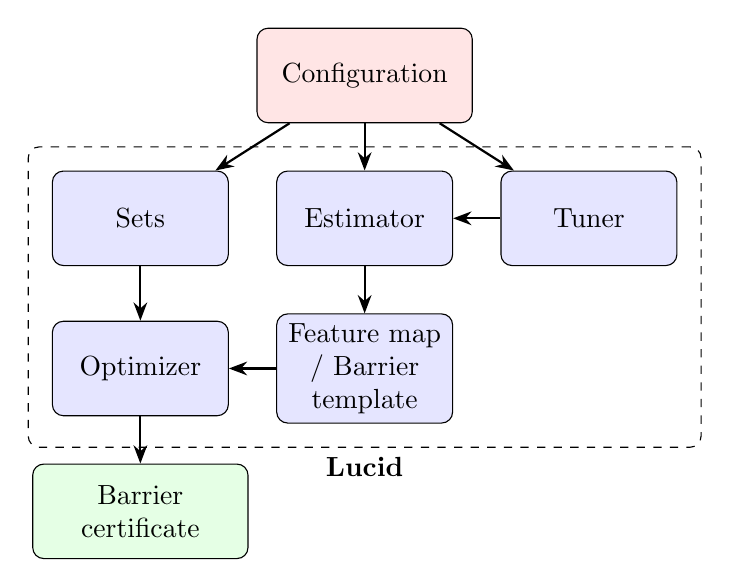
\begin{tikzpicture}[node distance=0.6cm and 0.6cm,
            input-block/.style={rectangle, draw, fill=red!10, text width=2.5cm, minimum height=1.2cm, align=center, rounded corners},
            output-block/.style={rectangle, draw, fill=green!10, text width=2.5cm, minimum height=1.2cm, align=center, rounded corners},
            block/.style={rectangle, draw, fill=blue!10, text width=2.0cm, minimum height=1.2cm, align=center, rounded corners},
            arrow/.style={thick,->,>=Stealth},
            tool/.style={rectangle, draw, fill=magenta!10, text width=3cm, minimum height=0.8cm, align=center, rounded corners},
            inv/.style={}
        ]

        % Input block
        \node[input-block] (input) {Configuration};

        % Lucid blocks
        \node[block, below=of input] (estimator) {Estimator};
        \node[block, right=of estimator] (tuner) {Tuner};
        \node[block, left=of estimator] (sets) {Sets};
        \node[block, below=of estimator] (feature) {Feature map / Barrier template};
        \node[block, left=of feature] (optimizer) {Optimizer};
        % \node[block, below=of optimizer] (verifier) {Verifier};
        \node[draw, dashed, inner sep=0.3cm, rounded corners,
        % fit=(estimator)(feature)(optimizer)(verifier), label=above:{\textbf{Lucid}}] {};
        fit=(estimator)(feature)(optimizer)(sets)(tuner), label=below:{\textbf{Lucid}}] {};

        % Output block
        % \node[output-block, left=of verifier] (output) {Barrier certificate};
        \node[output-block, below=of optimizer] (output) {Barrier certificate};

        % Smt solvers
        % \node[inv, below=2.5cm of verifier.north, anchor=north] (smtInv) {};
        % \node[tool, left=0.3cm of smtInv] (dreal) {dReal};
        % \node[tool, right=0.3cm of smtInv] (cvc5) {CVC5};
        % \node[draw, dashed, inner sep=0.3cm, rounded corners,
        % fit=(dreal)(cvc5), label=left:{\textbf{SMT Solver}}] {};

        % Arrows
        \draw[arrow] (input) -- (estimator);
        \draw[arrow] (input) -- (tuner);
        \draw[arrow] (input) -- (sets);
        \draw[arrow] (sets) -- (optimizer);
        \draw[arrow] (tuner) -- (estimator);
        \draw[arrow] (estimator) -- (feature);
        \draw[arrow] (feature) -- (optimizer);
        % \draw[arrow] (optimizer) -- (verifier);
        % \draw[arrow] (verifier) -- (output);
        \draw[arrow] (optimizer) -- (output);

        % \draw[arrow] (cvc5.north) -- (verifier.south);
        % \draw[arrow] (dreal.north) -- (verifier.south);

    \end{tikzpicture}
    \caption{General architecture of Lucid, highlighting its core components and their connections.}
    \label{fig:architecture}
\end{figure}


\paragraph{Literature Background.}
\todo{Add relevant literature citations and background information here.}

% \begin{figure}
    \centering
    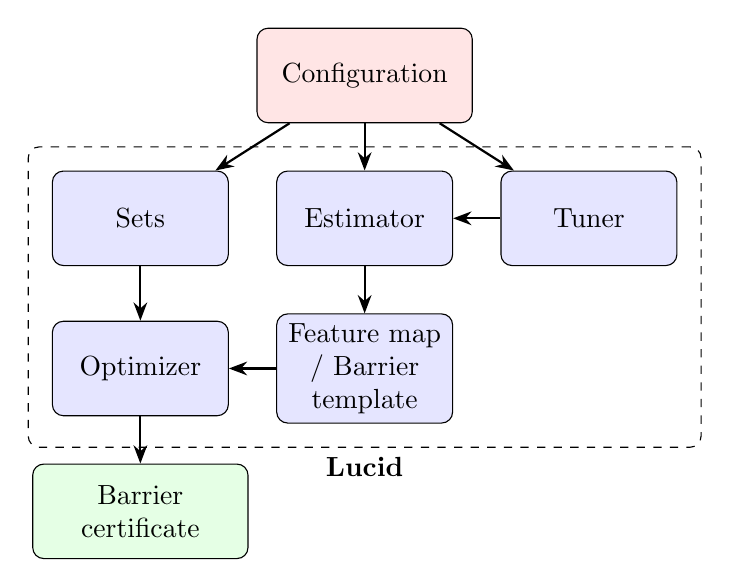
\begin{tikzpicture}[node distance=0.6cm and 0.6cm,
            input-block/.style={rectangle, draw, fill=red!10, text width=2.5cm, minimum height=1.2cm, align=center, rounded corners},
            output-block/.style={rectangle, draw, fill=green!10, text width=2.5cm, minimum height=1.2cm, align=center, rounded corners},
            block/.style={rectangle, draw, fill=blue!10, text width=2.0cm, minimum height=1.2cm, align=center, rounded corners},
            arrow/.style={thick,->,>=Stealth},
            tool/.style={rectangle, draw, fill=magenta!10, text width=3cm, minimum height=0.8cm, align=center, rounded corners},
            inv/.style={}
        ]

        % Input block
        \node[input-block] (input) {Configuration};

        % Lucid blocks
        \node[block, below=of input] (estimator) {Estimator};
        \node[block, right=of estimator] (tuner) {Tuner};
        \node[block, left=of estimator] (sets) {Sets};
        \node[block, below=of estimator] (feature) {Feature map / Barrier template};
        \node[block, left=of feature] (optimizer) {Optimizer};
        % \node[block, below=of optimizer] (verifier) {Verifier};
        \node[draw, dashed, inner sep=0.3cm, rounded corners,
        % fit=(estimator)(feature)(optimizer)(verifier), label=above:{\textbf{Lucid}}] {};
        fit=(estimator)(feature)(optimizer)(sets)(tuner), label=below:{\textbf{Lucid}}] {};

        % Output block
        % \node[output-block, left=of verifier] (output) {Barrier certificate};
        \node[output-block, below=of optimizer] (output) {Barrier certificate};

        % Smt solvers
        % \node[inv, below=2.5cm of verifier.north, anchor=north] (smtInv) {};
        % \node[tool, left=0.3cm of smtInv] (dreal) {dReal};
        % \node[tool, right=0.3cm of smtInv] (cvc5) {CVC5};
        % \node[draw, dashed, inner sep=0.3cm, rounded corners,
        % fit=(dreal)(cvc5), label=left:{\textbf{SMT Solver}}] {};

        % Arrows
        \draw[arrow] (input) -- (estimator);
        \draw[arrow] (input) -- (tuner);
        \draw[arrow] (input) -- (sets);
        \draw[arrow] (sets) -- (optimizer);
        \draw[arrow] (tuner) -- (estimator);
        \draw[arrow] (estimator) -- (feature);
        \draw[arrow] (feature) -- (optimizer);
        % \draw[arrow] (optimizer) -- (verifier);
        % \draw[arrow] (verifier) -- (output);
        \draw[arrow] (optimizer) -- (output);

        % \draw[arrow] (cvc5.north) -- (verifier.south);
        % \draw[arrow] (dreal.north) -- (verifier.south);

    \end{tikzpicture}
    \caption{General architecture of Lucid, highlighting its core components and their connections.}
    \label{fig:architecture}
\end{figure}


\section{Problem Statement}
\label{sec:problem-statement}

% Spaces and numbers
We denote the sets of positive integers and non-negative reals as $\N_{>0}$ and $\R_{\geq 0}$, respectively.
% Probability theory
Consider a Polish sample space $\X$ \cite{bogachev2007measure}.
Let $(\X,\borel{\X},\P)$ be the underlying probability space equipped with a Borel $\sigma$-algebra $\borel{\X}$ defined over $\X$, i.e., the smallest $\sigma$-algebra containing open subsets of $\X$, and a probability measure $\P$.
For a random variable $X$, let $p_X$ be the pushforward probability measure of $\P$ under $X$ such that $X\sim p_X(\cdotx)$.

The expected value of a function $f(X)$ on $\X$ is written as $\E_{p_X}[f(X)]$. If it is clear from the context, we abbreviate and write $\E[f(X)]$.
We denote the set of all probability measures for a given measurable space $(\X,\borel{\X})$ as $\mathcal{P}(\X)$.

The $n$-dimensional Gaussian measure with mean $\mu\in\mathbb{R}^n$ and covariance matrix $\Sigma\in\mathbb{R}^{n\times n}$ is given by
\begin{equation}
  \label{eq:gaussian-kernel}
  \mathcal N(dx|\mu, \Sigma) := \frac{dx}{ \sqrt{(2\pi)^n \left|\Sigma\right| }}\exp\left[-\frac{1}{2}(x-\mu)\T\Sigma^{-1\!}(x-\mu)\right],
\end{equation}
where $|\Sigma|$ is the determinant of $\Sigma$.
The Dirac delta measure $\delta_a:\borel{\X}\rightarrow [0,1]$ concentrated at a point $a\in\X$ is defined as $\delta_a(A)=1$ if $a\in A$ and $\delta_a(A)=0$ otherwise, for any measurable set $A\in\borel{\X}$.
We denote the uniform distribution over $\X$ as $\mathcal{U}_\X$ with realizations $x\sim\mathcal{U}_\X(\cdotx)$.

For two measurable spaces $(\X,\borel{\X})$ and $(\Y,\borel{\Y})$, a \emph{probability kernel} is a mapping $\p: \X \times \borel{\Y}\rightarrow  [0,1]$ such that $\p(X=x,\cdotx):\borel{\Y}\rightarrow[0,1]$ is a probability measure for all $x\in\X$, and $\p(\cdotx, B): \X\rightarrow [0,1]$ is measurable for all  $B\in\borel{\Y}$.
A probability kernel associates to each point $x\in\X$ a measure denoted by $\p(\cdotx|X=x)$.

% Linear algebra
The transpose of a vector or matrix $A$ is indicated as $A\T$.
Let the $N\times N$ dimensional identity matrix be given by $I_N$.
Let $X_N:=[x_i]_{i=1}^N$ be a column vector with $x_i\in\X$.
We denote the element-wise evaluation of a function $f:\X\rightarrow\R$ on $X_N$ as $f(X_N):=[f(x_i)]_{i=1}^N$.
Similarly, we may write $A = [a_{ij}]_{i,j=1}^N$ to denote a matrix with its elements.

\subsection{Discrete-Time Stochastic Systems}
In this work, we consider systems expressible as Markov decision processes over continuous state and input spaces, formally defined as follows.
\begin{definition}[Markov decision process (MDP)]
  An MDP is a tuple $\M=(\X,\X_0,\U,\Tr)$, comprising a state space $\X\subset\R^n$ with states $x\in\X$; initial states $x_0\in \X_0\subset\X$; an input space $\U$ with inputs $u\in\U$; and a probability kernel $\Tr:\X\times\U\times\borel{\X}\rightarrow[0,1]$.
\end{definition}

In every execution, given a current state $x\in\X$ and control input $u\in\U$, the MDP evolves to a consecutive state $x_{+}\in\X$, which is obtained as a realization $x_{+}\sim\Tr(\,\cdot\,|X=x,U=u)$.
As a notable class of systems that can be captured using MDPs, we may consider black-box systems with Markovian discrete-time stochastic dynamics, namely
\begin{equation}
  \label{eq:model}
  \M: \left\{ \begin{array}{ll}
    x_{t+1} & = f(x_t,u_t,w_t),\quad w_t\sim p_w(\cdotx), \\
    y_t     & = x_t,
  \end{array} \right.
\end{equation}
where the system state, control input, and observation at the $t^{\text{th}}$ time-step are denoted by $x_t$, $u_t$, and $y_t$, respectively.
The state evolution of the system, described by the function $f:\X\times\U\times\mathbb{W}\rightarrow\X$,
is subject to {independent, identically distributed (i.i.d.) noise} $w_t\sim p_w(\cdotx)$ supported on a set $\mathbb{W}$.

\paragraph{Implementation}

When using \lucid, the user needs to provide a set of sampled trajectories from the system.
This is often achieved by defining a function that takes as input the current state and control input and returns the next state, adding an i.i.d. noise sampled from an appropriate distribution, or it may be collected from a simulator or a real-world system.
The sampled trajectories are then fed into \lucid, either programmatically or through a file \todo{CSV, HDF5, other?}.
\todo{Allow a simple way to define the system model? Maybe latex2sympy?}
\todo{Graphical interface?}

\subsection{System Safety}
In this paper, we wish to synthesize a controller $\pi$ such that the closed-loop system $\pi\times\M$ is safe.
Particularly, we restrict our attention to \emph{stationary} policies of the form $\pi:\X\rightarrow\U$, as for MDPs there always exists a stationary policy that is optimal.
For an MDP $\M$, we characterize \emph{safety} as a property of its state. More precisely, a system $\pi\times\M$ is said to be safe if for any initial state $x_0\in \X_0$ the system does not enter an \emph{unsafe set} of states $\X_u\subset\X$.
Note that general stochastic systems do not admit a binary notion of safety.
Thus, we quantify the \emph{probability} of reaching $\X_u$ in a given finite horizon $T\in\N_{>0}$ and compute its complement.
A (finite-horizon) \emph{safety specification} $\psi_{\text{safe}:=(\X_u,T)}$ is hence fully characterized by an unsafe set $\X_u$ and a time horizon $T$.
The system $\pi\times\M$ satisfies $\psi_{\text{safe}}$ with probability at least $p\in(0,1)$ if the probability of its trajectories starting in $\X_0$ and avoiding $\X_u$ within horizon $T$ is at least $p$. This is denoted by $P^\pi_{\text{safe}}(\M):=\P(\pi\times\M\satisfies\psi_{\text{safe}})\geq p$~\cite{BK08}.

\paragraph{Implementation}

\lucid understands \texttt{RectSet}s and \texttt{Multiset}s \todo{PolytopeSet?}.
\todo{Set definition from file?}.
These are used to indicate the initial $\X_0$ set and unsafe set $\X_u$ when defining the safety specification $\psi_{\text{safe}}$.
Once the system is fully defined, the time horizon $T$ is set as a parameter of the verification process.
\todo{Support other kinds of properties other than safety (e.g., reachability)?}

\subsection{Control Barrier Certificates}
\label{sec:cbc}
Whilst certifying the safety of a stochastic system is generally challenging, \emph{control barrier certificates} (CBCs) and \emph{control barrier functions} (CBFs) leverage the concept of set invariance to arrive at an abstraction-free formulation. This has made CBCs/CBFs popular tools for safety verification and synthesis~\cite{prajna2006barrier,cosner2023generative}.
We briefly recall the definition of a \gls{cbc}.
\begin{definition}[Control barrier certificate (CBC)]\label{def:cbc}
  A function $\B:\X\rightarrow\R_{\geq 0}$ is called a \gls{cbc} of an MDP $\M=(\X,\X_0,\U,\Tr)$ with reference to an unsafe set $\X_u$, if we have
  \begin{itemize}
    \item[(a)] $\forall x_0\in \X_0\!:\,\B(x_0)\leq\eta$;
    \item[(b)] $\forall x_u\in \X_u\!:\,\B(x_u)\geq\gamma$; and
    \item[(c)] $\forall x\in\X,\exists u\in\U\!:\,\E_{\Tr}[\,\B(X^+)\mid X=x,\,U=u\,] -\B(x) \leq  c;$
  \end{itemize}
  for some constants $\gamma>\eta\geq0$ and $c\geq 0$.
\end{definition}
If one can find a \gls{cbc} for a system $\M$, then, a lower bound on the probability of $\M$ being safe is given by the following proposition due to \cite{kushner1967stochastic}.
\begin{proposition}[Finite-horizon safety]
  \label{prop:reach}
  Consider an MDP $\M=(\X,\X_0,\U,\Tr)$ and a safety specification $\psi_{\text{safe}}=(\X_u,T)$. Suppose there exists a CBC $B$ w.r.t. $\X_u$ (Definition~\autoref{def:cbc}) with constants $\eta$, $\gamma$, and $c$. Then, there exists a stationary policy $\pi$ such that
  $$P^\pi_{\text{safe}}(\M)\geq 1- \frac{\eta + cT}{\gamma}.$$
\end{proposition}

\paragraph{Implementation}

When verifying the safety of a system, \lucid will search for a \gls{cbc} $\B$ that satisfies the conditions in Definition~\ref{def:cbc}.
If it finds it, it will return the constants $\eta$, $\gamma$, and $c$, as well as the CBC $\B$ itself, which becomes a certificate of safety for the system $\M$.
The template of the barrier function is explored later in section~\ref{sec:benchmarks}.

\subsection{Kernel Mean Embeddings}

A symmetric function $k_\X:\X\times\X\rightarrow\R$ is called a (positive definite) \emph{kernel} (note the distinction from \emph{probability kernels}) if for all $N\in\N_{>0}$ we have $\sum_{i=1}^{N}\sum_{j=1}^{N}a_i a_j\allowbreak k_\X(x_i,x_j) \geq 0$ for $x_1,\ldots,x_N\in\X\subset{\R^n}$ and $a_1,\ldots,a_N\in\R$.
A prominent example is the \emph{squared exponential} (SQExp) kernel \cite{Rasmussen2005GP,Kanagawa2018GPvsKernel}:
\begin{equation}
  \label{eq:gaussian-kernel}
  k_\X(x,x') := \sigma_f^2 \exp\left( -\frac{1}{2} (x-x')\T \Sigma\, (x-x') \right),\quad \Sigma:=\diag(\sigma_l)^{-2},
\end{equation}
with amplitude $\sigma_f^2\geq0$ and lengthscale coefficients $\sigma_l\in\R^n$.
%In the following, we refer to a positive definite kernel as \emph{kernel}, for simplicity.
For this work, we assume that all kernels are bounded on their domain, i.e., $\E_{}[k_\X(x,x)]<\infty$, $x\in\X$.
Given a kernel $k_\X$ on a non-empty set $\X$, there exists a unique corresponding \emph{reproducing kernel Hilbert space} (RKHS) $\Hilbert_{k_\X}$ of functions $f:\X\rightarrow\R$ equipped with an inner product $\innerH{\cdotx}{\cdotx}{\Hilbert_{k_\X}}$ possessing the \emph{reproducing property} such that for any function $f\in\Hilbert_{k_\X}$ and $x\in\X$ we have $f(x)=\innerH{f}{k_\X(\cdotx,x)}{\Hilbert_{k_\X}}$.
Note that $k_\X(\cdotx,x):\X\rightarrow\Hilbert_{k_\X}$ is a real-valued function,
\new{which is} also called an implicit \emph{canonical} \emph{embedding} or \emph{feature map} $\phi_\X$
such that $k_\X(x,x')=\innerH{\phi_\X(x)}{\phi_\X(x')}{\Hilbert_{k_\X}}$ for all $x,x'\in\X$.
For an RKHS $\Hilbert_{k_\X}$, we use the associated feature map $\phi_\X$ and kernel $k_\X$ interchangeably for ease of notation and comprehensibility.
%We will call the kernel associated to an RKHS $\Hilbert_{k_\X}$ the \emph{characteristic} kernel of $\Hilbert_{k_\X}$ and use $\phi_\X$ and $k_\X$ interchangeably for ease of notation and comprehensibility.
%and an implicit \emph{canonical} \emph{embedding} or \emph{feature map} $\phi_\X:\X\rightarrow\Hilbert_{k_\X}$ with an inner product on $\Hilbert_{k_\X}$, i.e., $k_\X(x,x')=\innerH{\phi_\X(x)}{\phi_\X(x')}{\Hilbert_{k_\X}}$, 
%Furthermore, 
The inner product induces the norm $\norm{f}_{\Hilbert_{k_\X}}\!\!\!\!:=\!\!\sqrt{\smash[b]{\innerH{f}{f}{\Hilbert_{k_\X}}}}$ of the RKHS.
%Note that $\Hilbert_{k_\X}$ is a space of functions $f:\X\rightarrow\R$. 
%It is equipped with the infamous \emph{reproducing property} such that for any function $f\in\Hilbert_{k_\X}$ and $x\in\X$ we have $f(x)=\innerH{f}{\phi_\X(x)}{\Hilbert_{k_\X}}$.
%Furthermore, the norm associated with the RKHS $\Hilbert_{k_\X}$ is defined as $\norm{f}_{\Hilbert_{k_\X}}:=\sqrt{\innerH{f}{f}{\Hilbert_{k_\X}}}$.
%We refer the interested reader to XX for a comprehensive dissemination on RKHS.
Throughout this paper, we assume that all RKHSs are \emph{separable}.
Given $N$ i.i.d. samples $\hat X_N:=[\hat{x}_i]_{i=1}^N$ with $\hat{x}_i\in\X$, the
\emph{Gram matrix} of $k_\X$ is given by
$K_{\hat{X}}^N:=[k_\X(\hat{x}_i,\hat{x}_j)]_{i,j=1}^N.$
Furthermore, we define the vector-valued function
$k_{\hat{X}}^N(x)  := [k_\X(x,\hat{x}_i)]_{i=1}^N.$

\subsection{Data-Driven Barrier Formulation}
\label{sec:data-driven-barrier-formulation}
Compared to the typical spatial form \eqref{eq:representer-form} based on spatial support vectors $\bar{x}_1,\bar{x}_2,\ldots\in\X$, the spectral form \eqref{eq:representer-form-spectral} is a much more efficient representation for higher-dimensional systems.
The number of spatial support vectors needed to construct adequately expressive barriers grows exponentially in the dimensionality of the system. We avoid this.

Apart from the memory efficiency of the spectral barrier form, we can apply the same idea to collapse the complex CME term in \eqref{eq:semiinf-prog-kushner} via the \emph{fast Fourier transform} (FFT). That is we obtain spectral coefficients $H\in\R^{(2M+1)\times (2M+1)}$ s.t.
\begin{equation}
  k^N_{\hat{X}}(x)\T\left[ K^N_{\hat{X}}+N\lambda I_N\right]^{-1\!} (\Phi_{M, \hat{X}^{+\!}}^{N})\T b \approx \phi_M(x)\T H b,\label{eq:cme-term-spectral-approx}
\end{equation}
where $\Phi_{M, \hat{X}^{+\!}}^{N} := [\phi_M(\hat{x}^+_1),\ldots,\phi_M(\hat{x}^+_N)]$.
Whilst projection onto a truncated Fourier basis introduces an approximation error, the error decreases exponentially with the cardinality of wavenumbers in the basis \cite{rahimi2007random}.
% Our numerical results suggest that the empirical error is negligible.


Substituting the barrier $B\in\Hilbert_M$ of the form \eqref{eq:representer-form-spectral} and the approximation of the CME term in \eqref{eq:cme-term-spectral-approx} into the SIP \eqref{eq:semiinf-prog}, we obtain the \emph{semi-infinite linear program} (SILP)
\begin{subequations}
  \begin{align}
    \min_{b, c, \eta, \gamma} \; & \frac{\eta + cT}{\gamma},\label{eq:semiinfLP-prog-objective}                                                 \\
    \text{s.t.}\quad
                                 & \forall x_0\in\X_0:\,\phi_M(x_0)\T b\leq\eta,\label{eq:semiinfLP-prog-initial}                               \\
                                 & \forall x_u\in\X_u:\,\phi_M(x_u)\T b\geq\gamma,\label{eq:semiinfLP-prog-unsafe}                              \\
                                 & \forall x\in\X: \, \phi_M(x)\T (H b - b) \leq c - \varepsilon\bar{B}\kappa,\label{eq:semiinfLP-prog-kushner} \\
                                 & \forall x\in\X:\,\phi_M(x)\T b\geq 0,\label{eq:semiinfLP-prog-positive}                                      \\
                                 & c\geq 0,\,\gamma>\eta\geq 0,\,b\in\R^{2M+1},\nonumber
  \end{align}\label{eq:semiinfLP-prog}%
\end{subequations}
with coefficients $\kappa\geq\sigma_f$ and $\bar{B}\geq\norm{b}_2$.

\subsection{Finite-Constraint Relaxation}\label{sec:finite-constraint-relaxation}
There exist results that establish deterministic sampling-based bounds for multivariate trigonometric polynomials \cite{cifuentes2017sampling,pfister2018bounding} that can be applied to the bandlimited spectral barrier in \eqref{eq:representer-form-spectral}. This allows us to relax the SILP \eqref{eq:semiinfLP-prog} to a \emph{linear program} (LP) with finitely many constraints by sampling a finite set
$X_{\hat{N}} \subset\X$ of cardinality $\hat{N}$.
By choosing $\hat{N}=Q^n$ equidistant points that form a discrete lattice of points to cover the (state) space, the corresponding constraints can be efficiently evaluated in $\mathcal{O}(Q\log(Q))$ operations using the inverse FFT.
Note that this also substantially reduces the number of evaluations of the computationally expensive CME term in \eqref{eq:semiinf-prog-kushner}, which requires $\mathcal{O}(N^2)$ operations per evaluation. Refer to the Petersen-Middleton theorem \cite{petersen1962sampling}, which generalizes the Nyquist-Shannon sampling theorem to higher-dimensional Euclidean spaces, for further details.

We use the following result by \cite{pfister2018bounding}.
\begin{lemma}[Trigonometric bounds]\label{lem:trig-bound}
  Consider a real-valued trigonometric polynomial $f:[0,1]^n\rightarrow\R$ (cf. \eqref{eq:representer-form-spectral}) with maximum degree $d\in\N_{\geq 0}$ and a sampling lattice $\Theta_Q:=\{\frac{2\pi l}{Q},\, l=0,\ldots,Q-1\}$ with $Q\geq 2d+1$.
  Let $\bar{f}_{Q^n}:=\max_{z\in\Theta^n_Q} f(z)$ and $\underbar{f}_{Q^n}:=\min_{z\in\Theta^n_Q} f(z)$. Then, we have that
  \begin{equation*}
    \frac{1}{2}\big(\bar{f}_{Q^n} + \underbar{f}_{Q^n} - C_{Q^n}\left(\bar{f}_{Q^n}-\underbar{f}_{Q^n}\right)\big)
    \leq
    f(z)
    \leq
    \frac{1}{2}\big(\bar{f}_{Q^n} + \underbar{f}_{Q^n} + C_{Q^n}\left(\bar{f}_{Q^n}-\underbar{f}_{Q^n}\right)\big),
  \end{equation*}
  with a coefficient given by
  \setlength{\belowdisplayskip}{3pt}
  \begin{equation*}
    C_{Q^n} := \left(1-\frac{2d}{Q}\right)^{-\frac{n}{2}}.
  \end{equation*}
\end{lemma}
% \Oliver{The paper \cite{pfister2018bounding} provides a more complex expression for $C_{Q^n}$ that I put as [...]. They also provide the upper bound I use so far.}


Via Lemma~\ref{lem:trig-bound}, we obtain a finite-constraint relaxation of the SIP \eqref{eq:semiinf-prog} based on the constraint-tightening reasoning
\begin{equation*}
  \frac{1}{2}\big(\mathrm{max}_{\hat{N}}^\X + \mathrm{min}_{\hat{N}}^\X - C_{\hat{N}}\left(\mathrm{max}_{\hat{N}}^\X-\mathrm{min}_{\hat{N}}^\X\right)\big)\geq \mathrm{lb}
  \quad\Longrightarrow\quad
  \forall x\in\X: f(x) \geq \mathrm{lb},
\end{equation*}
where $\mathrm{max}_{\hat{N}}^\X:=\max_{x\in X_{\hat{N}}} \left\lbrace\phi_M(x)\T b\right\rbrace$ and $\mathrm{min}_{\hat{N}}^\X:=\min_{x\in X_{\hat{N}}} \left\lbrace\phi_M(x)\T b\right\rbrace$ for some desired lower bound $\mathrm{lb}\in\R$.
Thus, we obtain strengthened constraints of the form
\begin{align*}
  \mathrm{min}_{\hat{N}}^\X \geq \frac{2}{C_{\hat{N}}+1}\mathrm{lb} + \frac{C_{\hat{N}}-1}{C_{\hat{N}}+1}\mathrm{max}_{\hat{N}}^\X.
\end{align*}
We obtain an analogous constraints for an upper bound $\forall x\in\X: f(x) \leq \mathrm{ub}$.

\paragraph{Implementation}

The finite-constraint relaxation of the SIP \eqref{eq:semiinf-prog} is what \lucid uses to synthesize the \gls{cbc} $\B$.
More precisely, we follow the steps outlined in~\autoref{fig:steps}.
While the theory gives us precise indication on how to construct the \gls{lp} which would yield a correct-by-design solution,
in practice the problem may become too conservative.
To mitigate this, we can either increase the number of lattice points $Q$, worsening the computational efficiency, 
or we may choose to adjust the coefficient $C_{\hat{N}}$, improving performance at the cost of loosening the guarantees, 
which can still be checked with the verifier, provided we have access to the system's model.

\begin{figure}[ht]
    \centering
    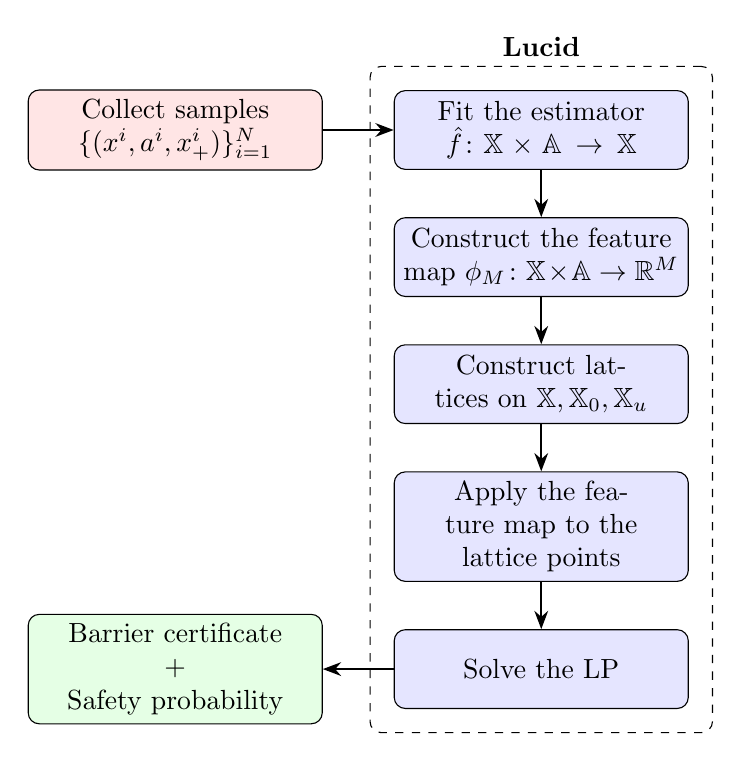
\begin{tikzpicture}[node distance=0.6cm and 0.9cm,
            input-block/.style={rectangle, draw, fill=red!10, text width=3.5cm, minimum height=1.0cm, align=center, rounded corners},
            output-block/.style={rectangle, draw, fill=green!10, text width=3.5cm, minimum height=1.0cm, align=center, rounded corners},
            block/.style={rectangle, draw, fill=blue!10, text width=3.5cm, minimum height=1.0cm, align=center, rounded corners},
            arrow/.style={thick,->,>=Stealth},
            tool/.style={rectangle, draw, fill=green!20, text width=2cm, minimum height=0.8cm, align=center, rounded corners},
            inv/.style={}
        ]

        % Input block
        \node[input-block] (input) {Collect samples $\{(x^i,a^i, x_+^i)\}_{i=1}^N$};

        % Lucid blocks
        \node[block, right=of input] (estimator) {Fit the estimator $\hat{f}\colon \X\times\A \to \X$};
        \node[block, below=of estimator] (feature) {Construct the feature map $\phi_M\colon \X\times\A \to \mathbb{R}^M$};
        \node[block, below=of feature] (lattice) {Construct lattices on $\X, \X_0, \X_u$};
        \node[block, below=of lattice] (apply-lattice) {Apply the feature map to the lattice points};
        \node[block, below=of apply-lattice] (optimizer) {Solve the LP};
        \node[draw, dashed, inner sep=0.3cm, rounded corners,
        fit=(estimator)(feature)(lattice)(apply-lattice)(optimizer), label=above:{\textbf{\lucid}}] {};

        % Output block
        \node[output-block, left=of optimizer] (output) {Barrier certificate\\+\\Safety probability};

        % Arrows
        \draw[arrow] (input) -- (estimator);
        \draw[arrow] (estimator) -- (feature);
        \draw[arrow] (feature) -- (lattice);
        \draw[arrow] (lattice) -- (apply-lattice);
        \draw[arrow] (apply-lattice) -- (optimizer);
        \draw[arrow] (optimizer) -- (output);

    \end{tikzpicture}
    \caption{Sequence of steps \lucid goes through to generate a barrier certificate.}
    \label{fig:steps}
\end{figure}


\subsection{Tuning the Hyperparameters}
\label{sec:tuning-hyperparameters}

Kernel methods do not require the expensive learning process of other machine learning methods, such as neural networks.
However, they still depend on a number of \hp, such as the kernel bandwidth $\sigma_f$ and the number of Fourier coefficients $M$.
Changes in their values can have a significant impact on the estimator's efficiency and accuracy.
The process of finding good values for these \hp is known as \emph{hyperparameter tuning}, and it is problem-dependent.

There are several approaches to find the optimal \hp for a given problem.
A cheap option which can be used as a starting point when working with a Gaussian Kernels as in~\eqref{eq:gaussian-kernel} is to use the \emph{median heuristic} \cite{garreau2018largesampleanalysismedian}.
We choose $\sigma_l^2$ to be the median of the squared distances between all pairs of points in the training set, i.e.,
\begin{equation}
  \sigma_l^2 = \mathrm{median}_{1 \leq i < j \leq N}\left(\|\hat{x}_i-\hat{x}_j\|^2\right),
\end{equation}
where $\hat{x}_1,\ldots,\hat{x}_N$ are the $N$ training samples.
If $N(N-1)/2$ is even, the median is the average of the two middle values in the sorted list of distances.
Better results can be obtained via \emph{grid search}, which consists of evaluating the performance of the estimator for all combinations of \hp in a predefined grid.
This approach is simple to implement and can be very effective for small problems, but it can become computationally expensive for larger problems.
Borrowing a technique from Gaussian processes, we can also try to optimize the \hp to maximize the \emph{log marginal likelihood}, defined as
\begin{equation}
  \log p(\hat{X^+}_N | \hat{X}_N) = - \frac{1}{2}\hat{X^+}_N\T (K_{\hat{X}}^N + N\lambda I_N)^{-1} \hat{X^+}_N -\frac{1}{2}\log |K_{\hat{X}}^N + N\lambda I_N| - \frac{N}{2}\log(2\pi).
\end{equation}

\paragraph{Implementation}

While it is possible to tune the \hp with any method and then set them manually in the estimator, \lucid provides a set of classes, which specialize the \texttt{Tuner} interface, to automate the process.
The \texttt{GridSearchTuner} class implements the grid search method, while the \texttt{MedianHeuristicTuner} class implements the median heuristic.
If the user wants to optimize the log marginal likelihood, they can use the \texttt{LBGSTuner} class, which runs the L-BFGS or L-BFGS-B quasi-Newton optimization algorithms~\cite{book:nonlinear-programming} over the log marginal likelihood function.
Internally, \lucid uses the \texttt{LBFGS++} library~\footnote{https://github.com/yixuan/LBFGSpp} to perform the optimization.

\section{Tool Evaluation}
\label{sec:evaluation}

We evaluate \lucid on a set of benchmarks, which are described in detail in the documentation.

\paragraph{Linear System}

To showcase the basic functionality of \lucid, we consider a simple linear system with the dynamics

\begin{equation*}
  \begin{bmatrix}
    {x}_{1, t+1}
  \end{bmatrix}
  = \begin{bmatrix}
    0.5
  \end{bmatrix}
  \begin{bmatrix}
    {x}_{1, t}
  \end{bmatrix} + w_t,
\end{equation*}
where $w_t\sim\mathcal{N}(\cdotx\vert 0,0.01I)$ is a one-dimensional Gaussian noise.
We restrict the state space to the interval $\X=[-1,1]$ and define the initial set $\X_0=[-0.5,0.5]$ and the unsafe set $\X_u=[-1,-0.9]\cup[0.9,1]$.
Translating the system into the \lucid format, we obtain the following configuration file:
\lstinputlisting[language=Python,caption={\texttt{linear.py} configuration file.}]{code/linear.py}
It can then be run with the command
\begin{lstlisting}[language=bash]
python -m pylucid tests/bindings/pylucid/MinScenarioConfig.py --seed 42 --gamma 1.0 \
  --time_horizon 5 --num_samples 1000 --lambda 1e-3 --sigma_f 15.0 \ 
  --sigma_l 1.75555556 --num_frequencies 4 --plot --verify --oversample_factor 32.0
\end{lstlisting}
to produce the results shown in~\autoref{fig:linear}.
By including the \texttt{--verify} flag, also get formal guarantees that the barrier is indeed a valid \gls{cbc} for the system.
\begin{lstlisting}[language=bash]
# ...
[info] [thread 1] [-] The barrier has been verified via dReal
# ...
\end{lstlisting}

\begin{figure}[ht]
  \import{fig}{linear.pgf}
  \caption{\gls{cbc} synthesis for the linear system benchmark.
    The blue regions represent the initial set $\X_0$, while the red regions represent the unsafe set $\X_u$.
    The pink surface indicates the value of $\gamma$.
  }
  \label{fig:linear}
\end{figure}

\paragraph{Barrier 3}

The first benchmark is inspired by the example \barr from \cite{abate2021fossil}, which we extend by adding stochastic noise $w_t\sim\mathcal{N}(\cdotx\vert 0,0.01I_2)$ to arrive at the two-dimensional nonlinear stochastic dynamics
\begin{equation*}
  \begin{bmatrix}
    {x}_{1, t+1} \\
    {x}_{2, t+1}
  \end{bmatrix}
  = \begin{bmatrix}
    {x}_{2, t} \\
    \frac{1}{3} {x}^3_{1, t} - {x}_{1,t} - {x}_{2,t}
  \end{bmatrix} + w_t.
\end{equation*}
We illustrate the setup in Figure~\ref{fig:CSBarr3}.

The goal is to compute the probability that the system initialized in $[{x}_{1,0},{x}_{2,0}]\T\in \X_0$ (blue regions) does not enter the unsafe regions $\X_u$ (in red) within $T=10$ time steps.

\begin{figure}[ht]
  \import{fig}{barrier3.pgf}
  \caption{\gls{cbc} synthesis for the \barr benchmark.
    The blue regions represent the initial set $\X_0$, while the red regions represent the unsafe set $\X_u$.
    The pink surface indicates the value of $\gamma$.
  }
  \label{fig:CSBarr3}
\end{figure}


\section*{Acknowledgements}
The authors thank \dots.

\bibliographystyle{ieeetr}
\bibliography{resources}

\newpage
% !TEX root =  main.tex
\appendix

% \section{Additional Theoretical Details}
% \paragraph{RKHS basics.}
% A symmetric function $k_\X:\X\times\X\rightarrow\R$ is called a (positive definite) \emph{kernel} (note the distinction from \emph{probability kernels}) if for all $N\in\N_{>0}$ we have $\sum_{i=1}^{N}\sum_{j=1}^{N}a_i a_j\allowbreak k_\X(x_i,x_j) \geq 0$ for $x_1,\ldots,x_N\in\X\subset{\R^n}$ and $a_1,\ldots,a_N\in\R$.
% A prominent example is the \emph{squared exponential} (SQExp) kernel \shortcite{Rasmussen2005GP,Kanagawa2018GPvsKernel}:
% \begin{equation}
%     k_\X(x,x') := \sigma_f^2 \exp\left( -\frac{1}{2} (x-x')\T \Sigma\, (x-x') \right),\quad \Sigma:=\mathrm{diag}(\sigma_l)^{-2},\label{eq:sqexp_kernel}
% \end{equation}
% with amplitude $\sigma_f^2\geq0$ and lengthscale coefficients $\sigma_l\in\R^n$.
% \new{For this work,} we assume that all kernels are bounded on their domain, i.e., $\E_{}[k_\X(x,x)]<\infty$, $x\in\X$.
% Given a kernel $k_\X$ on a non-empty set $\X$, there exists a unique corresponding
% \emph{reproducing kernel Hilbert space} (RKHS) $\Hilbert_{k_\X}$
% of functions $f:\X\rightarrow\R$ equipped with an inner product $\innerH{\cdotx}{\cdotx}{\Hilbert_{k_\X}}$
% with the celebrated \emph{reproducing property} such that for any function $f\in\Hilbert_{k_\X}$ and $x\in\X$ we have $f(x)=\innerH{f}{k_\X(\cdotx,x)}{\Hilbert_{k_\X}}$.
% Note that $k_\X(\cdotx,x):\X\rightarrow\Hilbert_{k_\X}$ is a real-valued function,
% which is also called an implicit \emph{canonical} \emph{embedding} or \emph{feature map} $\phi_\X$
% such that $k_\X(x,x')=\innerH{\phi_\X(x)}{\phi_\X(x')}{\Hilbert_{k_\X}}$ for all $x,x'\in\X$.
% For an RKHS $\Hilbert_{k_\X}$, we use the associated feature map $\phi_\X$ and kernel $k_\X$ interchangeably for ease of notation and comprehensibility.
% The inner product induces the norm $\norm{f}_{\Hilbert_{k_\X}}\!\!\!\!:=\!\!\sqrt{\smash[b]{\innerH{f}{f}{\Hilbert_{k_\X}}}}$ of the RKHS. 
% Throughout this paper, we assume that all RKHSs are \emph{separable}.
% Refer to the monograph by \citet{Berlinet2004RKHSProbStat} for a comprehensive study on RKHSs.
% Given $N$ i.i.d. samples $\hat X_N:=[\hat{x}_i]_{i=1}^N$ with $\hat{x}_i\in\X$, the
% \emph{Gram matrix} of $k_\X$ is given by
% $\new{K_{\hat{X}}^N}:=[k_\X(\hat{x}_i,\hat{x}_j)]_{i,j=1}^N.$
% Furthermore, we define the vector-valued function 
% $\new{k_{\hat{X}}^N}(x)  := [k_\X(x,\hat{x}_i)]_{i=1}^N.$

% \begin{definition}[Conditional Mean Embedding (CME)]\label{def:condMeanEmbed}
%     Given two RKHSs $\Hilbert_{k_\X}$ and $\Hilbert_{k_\Y}$ with the associated kernels $k_\X\colon\X\times\X\to\R$ and $k_\Y\colon\X\times\X\to\R$, the \emph{CME} of a probability kernel $\Tr\colon\X\times\borel{\Y}\rightarrow[0,1]$ is an $X$-measurable random variable taking values in $\Hilbert_{k_\Y}$, given by
%     \begin{equation*}
%         \cme_{k_\Y|k_\X}(\Tr)(\cdotx) := \E_{\Tr}[\phi_\Y(Y)\mid X=\cdotx].
%     \end{equation*}
% \end{definition}

\section{Linear Program}
The finitely-constrained LP discussed in Section~\ref{sec:ddbarriers} is presented. For this, the lattices $X_{{N}}\subset\X$, $\smash{\{ x_0^{1}, \ldots, x_0^{{N}_0} \}} \subset \X_0$, and $\smash{\{ x_u^{1}, \ldots, x_u^{{N}_u} \}} \subset \X_u$ of cardinality ${N}_0\in\N$ and ${N}_u\in\N$, respectively, are formed.
%
For given values of $\overline{\B}$, $\gamma$, and robustness radius $\mathcal{R}\geq0$, the following LP is obtained:
\begin{equation*}
      \begin{alignedat}{3}
                  & \min_{\stackrel{b, c, \eta}{\Bmin_{{N}}^{\X_0}, \Bmax_{{N}}^{\X_u},\Bmax_{{N}}^\X,\Bmin_\Delta}}\hspace{-1.5em} &                                          & \eta + cT,                                    &                   &
            %\label{eq:blackbox:linear_prog_objective}
            \\
                  & \text{subject to}
                  &                                                                                                                 & \phi_M(x_0^{i})\T b\leq\hat{\eta}, \quad &                                               & i=1,\ldots,{N}_0,
            %\label{eq:blackbox:linear_prog_initial}
            \\
                  &                                                                                                                 &                                          & \phi_M(x_u^{i})\T b\geq\hat{\gamma},
            \quad &                                                                                                                 & i=1,\ldots,{N}_u,
            %\label{eq:blackbox:linear_prog_unsafe}
            \\
                  &                                                                                                                 &                                          & \phi_M(x^{i})\T(Hb - b) \leq \hat{\Delta},
            \quad &                                                                                                                 & i=1,\ldots,{N},
            %\label{eq:blackbox:linear_prog_kushner}
            \\
                  &                                                                                                                 &                                          & \phi_M(x^{i})\T b\geq \hat{\xi},
            \quad &                                                                                                                 & i=1,\ldots,{N},
            %\label{eq:blackbox:linear_prog_positive}
            \\
                  &                                                                                                                 &                                          & \Bmin_{{N}}^{\X_0}\leq\phi_M(x_0^{i})\T b,
            \quad &                                                                                                                 & i=1,\ldots,{N}_0,                                                                                              \\
                  &                                                                                                                 &                                          & \Bmax_{{N}}^{\X_u}\geq\phi_M(x_u^{i})\T b,
            \quad &                                                                                                                 & i=1,\ldots,{N}_u,                                                                                              \\
                  &                                                                                                                 &                                          & \Bmax_{{N}}^\X\geq\phi_M(x^{i})\T b,
            \quad &                                                                                                                 & i=1,\ldots,{N},                                                                                                \\
                  &                                                                                                                 &                                          & \Bmin_\Delta\leq\phi_M(x^{i})\T (Hb - b),
            \quad &                                                                                                                 & i=1,\ldots,{N},                                                                                                \\
                  &                                                                                                                 &                                          & c\geq 0,\,\gamma>\eta\geq 0,\, b\in\R^{2M+1}, &                   &
            \label{eq:blackbox:linear_prog}%
      \end{alignedat}
\end{equation*}
with $\overline{\kappa}\geq\sigma_f$, $\overline{\B}\geq\norm{b}_2$, and constraint-tightening coefficients
\begin{align*}
      \hat{\eta}   & := \frac{2}{C_{{N}}+1}\eta + \frac{C_{{N}}-1}{C_{{N}}+1}\Bmin_{{N}}^{\X_0},
      \\                                                                                                                                    & \hat{\gamma} := \frac{2}{C_{{N}}+1}\gamma + \frac{C_{{N}}-1}{C_{{N}}+1}\Bmax_{{N}}^{\X_u}, \\
      \hat{\Delta} & := \frac{2}{C_{{N}}+1}\left(c - \mathcal{R}\overline{\B}\overline{\kappa}\right) + \frac{C_{{N}}-1}{C_{{N}}+1}\Bmin_\Delta,
      \\                                                                                                                                     & \hat{\xi} := \frac{C_{{N}}-1}{C_{{N}}+1}\Bmax_{{N}}^\X.
\end{align*}


% \section{Proofs}
% We have collected a series of proofs of the claims we made in the main text.

\section{Installation}
Provided \texttt{Python>=3.8} is already present, \pylucid can be installed with the command
\begin{lstlisting}[language=bash,numbers=none,xleftmargin=0em]
pip install pylucid[gui,plot] --index-url \
  https://gitlab.com/api/v4/projects/71977529/packages/pypi/simple
\end{lstlisting}
There are a few limitation some of the dependencies introduce, which may preclude the ability of using certain features on not supported platforms.
Formal verification of the barrier requires the \dreal SMT solver, which can only be installed on Linux and non-ARM macOS.
Support for \highs \gls{lp} is not available on Windows at the moment.
The \gurobi solver must be installed beforehand, and requires a license for commercial use, but is free for academic purposes.

For more details on the installation process, please refer to the online documentation at \url{https://lucidtoolsource.gitlab.io/lucid/md_docs_2Pylucid.html}.

\section{Benchmarks}
\label{app:benchmarks}
Complete list of results for the benchmarks presented in Section~\ref{sec:experiments}.
The legend is as follows:
\textit{Output} indicates the result produced by the solver (i.e., optimal, unbounded, infeasible or unspecified),
\textit{Prec} indicates the number of bits used in the last floating-point number representation,
\textit{Ref} indicates the number of refinements,
and \textit{time} is the time in seconds.

All benchmarks were run on a Windows 10 machine with an AMD Ryzen 9 5950X 16-Core Processor @ 3.40 GHz, and 64 GB of RAM, and all runs had the random seed set to $42$ to ensure reproducibility.
The scripts responsible for running the benchmarks and \hp tuning are available in the \texttt{benchmarks/integration} folder of the repository.
Note that a version of \texttt{Python>=3.9} is required to run the scripts, as some dependencies used to track the benchmarks' metrics across multiple runs are not compatible with \texttt{Python 3.8}.
The \hp tuning of the \estimator was performed with the \texttt{LbfgsTuner}, bounding the value of $\sigma_l$ between $[10^{-5}, 10^5]$, and refined with the \texttt{GridSearchTuner}.
The implementation can be found in the \texttt{benchmarks/integration/hp\_tuning.py} script. 
Note that we used the \gurobi optimiser.
Other optimizers, such as \alglib or \highs, can be used instead, but may yield different results, especially in terms of performance.

\subsection{Linear}

We consider the following system:
\begin{equation*}
    \begin{bmatrix}
        {x}_{t+1}
    \end{bmatrix}
    = \begin{bmatrix}
        0.5 {x}_{t}
    \end{bmatrix} + w_t,
\end{equation*}
where $w_t\sim\mathcal{N}(\cdotx\vert 0,0.01I_1)$.
Given
\begin{align*}
    &\X = [-1, 1] \\
    &\X_0 = [-0.5, 0.5] \\
    &\X_U = [-1, -0.9] \cup [0.9, 1],
\end{align*}
we want to ensure that the system, starting in $\X_0$, does not enter the unsafe regions $\X_U$ within $T=15$ time steps.
The complete configuration for the linear example benchmark is shown in Listing~\ref{lst:linear}.
\lstinputlisting[language=yaml,caption={Configuration for linear example},captionpos=b,label={lst:linear}]{code/linear.yaml}

\subsection{Barrier 2}

We consider the following system:
\begin{equation*}
    \begin{bmatrix}
        {x}_{1, t+1} \\
        {x}_{2, t+1}
    \end{bmatrix}
    = \begin{bmatrix}
        {x}_{2, t} - 1 + e^{-x_{1, t}} \\
        -\sin^2(x_{1, t})
    \end{bmatrix} + w_t,
\end{equation*}
where $w_t\sim\mathcal{N}(\cdotx\vert 0,0.01I_2)$.
Given
\begin{align*}
    &\X = [ -2, 2 ] \times [ -2 , 2 ] \\
    &\X_0 = \{ [x_1, x_2] : (x_1 + 0.5)^2 + (x_2 - 0.5)^2 \leq 0.4 \} \\
    &\X_U = \{ [x_1, x_2] : (x_1 - 0.7)^2 + (x_2 + 0.7)^2 \leq 0.3 \},
\end{align*}
we want to ensure that the system, starting in $\X_0$, does not enter the unsafe regions $\X_U$ within $T=5$ time steps.
The complete configuration for the \barrII benchmark is shown in Listing~\ref{lst:barrier2}.
\lstinputlisting[language=yaml,caption={Configuration for \barrII},captionpos=b,label={lst:barrier2}]{code/barrier2.yaml}

\subsection{Barrier 3}

We consider the following system:
\begin{equation*}
    \begin{bmatrix}
        {x}_{1, t+1} \\
        {x}_{2, t+1}
    \end{bmatrix}
    = \begin{bmatrix}
        {x}_{2, t} \\
        \frac{1}{3} {x}^3_{1, t} - {x}_{1,t} - {x}_{2,t}
    \end{bmatrix} + w_t,
\end{equation*}
where $w_t\sim\mathcal{N}(\cdotx\vert 0,0.01I_2)$.
Given
\begin{align*}
    &\X = [ -3, 2.5 ] \times [ -2 , 1 ] \\
    &\X_0 = [ 1 , 2 ] \times [ -0.7 , 0.3 ] \cup [ -1.8 , -1.4 ] \times [ -0.1 , 0.1 ] \\
    &\qquad \cup [-1.4, -1.2] \times [-0.5 , 0.1] \\
    &\X_U = [ 0.4 , 0.6 ] \times [ 0.2 , 0.6 ] \cup [ 0.6 , 0.7 ] \times [ 0.2 , 0.4 ],
\end{align*}
we want to ensure that the system, starting in $\X_0$, does not enter the unsafe regions $\X_U$ within $T=5$ time steps.
The complete configuration for the \barrIII benchmark is shown in Listing~\ref{lst:barrier3}.
\lstinputlisting[language=yaml,caption={Configuration for \barrIII},captionpos=b,label={lst:barrier3}]{code/barrier3.yaml}

\subsection{Overtaking}

We consider a scenario where an autonomous vehicle (AV) controlled by a \gls{nn} is overtaking another vehicle.
The dynamics of the ego vehicle are given by Dubin's car model \EC{does it need a cit or is it just textbook} by adding the noise vector $w = \begin{bmatrix}w_t^1 & w_t^2 & w_t^3\end{bmatrix}$ where each component is drawn from a zero-mean Gaussian with standard deviation $0.01$, $0.01$, and $0.001$, respectively.
The steering wheel angle is supplied by the \gls{nn} controller and we travel at a fixed velocity $v=1$.
Given
\todo{correct the sets}
\begin{align*}
    &\X = [ -3, 2.5 ] \times [ -2 , 1 ] \\
    &\X_0 = [ 1 , 2 ] \times [ -0.7 , 0.3 ] \cup [ -1.8 , -1.4 ] \times [ -0.1 , 0.1 ] \\
    &\qquad \cup [-1.4, -1.2] \times [-0.5 , 0.1] \\
    &\X_U = [ 0.4 , 0.6 ] \times [ 0.2 , 0.6 ] \cup [ 0.6 , 0.7 ] \times [ 0.2 , 0.4 ],
\end{align*}
we want to ensure that the system, starting in $\X_0$, does not enter the unsafe regions $\X_U$ within $T=5$ time steps.

The complete configuration for the \overtaking benchmark is shown in Listing~\ref{lst:overtaking}.
\lstinputlisting[language=yaml,caption={Configuration for \overtaking},captionpos=b,label={lst:overtaking}]{code/overtaking.yaml}


\end{document}

